\chapter{Traffic Characterization and Classification Evaluation}
\label{classification}
In this chapter, we will discuss how to collect the traffic of web applications in detail and present not only the traffic characterization of various web applications, but also the accuracy of their classification.

\section{Scenarios of Packet Collection}
\label{sec:scenario}
The network traffic is generated from user interactions on individual applications. We choose the following web applications for analysis: (1) Google docs for the office application, (2) Google map for the map application, (3) Youtube, Tudou, Dailymotion for the video streaming applications, (4) Google drive and Dropbox for the file transfer applications, and (5) Tetris Battle and Dungeon Rampage on Facebook for the game applications. In this work, we repeatedly performed the following actions ten times on either Chrome (version 41.0.2272.89) or Firefox (version 36.0.1) for a period from one to two minutes each time.

The interactions in the office application involve arbitrarily typing characters and changing the colors. The interactions in the map application involve typing an arbitrary location name to be searched in the map, zooming-in and zooming-out the map, and browsing the map. The interactions in the game application involve (1) arbitrarily moving a role and fighting with the other roles in Dungron Rampage and (2) moving and rotating the blocks in Tetris Battle. We also consider the download functions in the video streaming and the file sharing applications. In the former application, we typed an arbitrary video name and moved to a specific time position when watching a video or just silently watched a video until the end. In the latter application, we just downloaded an arbitrary file and waited silently until the completion of the file up/downloading.

\section{Traffic Characterization of Web Applications}
\label{sec:characterization}
A typical web session may involve several parallel connections to speed up fetching the requested content, and may also contain irrelevant connections such as those for advertisements. Thus, we manually inspected the content of requests and responses with the developer tools affiliated with the browsers when collecting the related packet traces, and focused only on the connections over which the user interactions are carried. To determine the connections associated with the user interactions, we watched the ongoing connection activities in the developer tool when interacting with a web application, and selected the longest one of these active connections as the main connection. Table~\ref{table:num_connection} presents the average number of connections and the standard deviation in each web application. The values demonstrate that Chrome creates more connections than Firefox on average to transfer the data for the same web applications. 

\begin{table}[h]
\centering
\caption{The average number of connections and the standard deviation (SD) for each web application.}
\label{table:num_connection}
\begin{tabular}{|l|l||l|l||l|l|}
\hline
\multicolumn{2}{|l||}{}                                                                                                                & \multicolumn{2}{l||}{Chrome} & \multicolumn{2}{l|}{Firefox} \\ \hline
Label                                                                     & Web application & Avg.   & SD     & Avg.    & SD   \\ \hline \hline
Document                                                                  & Google doc      & 37.30  & 4.69   & 33.70   & 2.71 \\ \hline
Map                                                                       & Google map      & 27.60  & 2.50   & 19.40   & 1.65 \\ \hline
\multirow{2}{*}{Game}                                                     & \begin{tabular}[c]{@{}l@{}}Dungeon\\ Rampage\end{tabular} 
                  & 125.40 & 10.01  & 108.30  & 7.45 \\ \cline{2-6} 
                                                                     & Tetris Battle   & 218.30 & 14.77  & 174.70  & 8.65 \\ \hline
\multirow{2}{*}{\begin{tabular}[c]{@{}l@{}}File \\ Transfer\end{tabular}} & Google Drive                                              
                  & 37.50  & 3.17   & 31.70   & 0.95 \\ \cline{2-6} 
                                                                        & Dropbox         & 68.00  & 11.26  & 61.30   & 3.30 \\ \hline
\multirow{3}{*}{\begin{tabular}[c]{@{}l@{}}Video \\ Stream\end{tabular}}  & Youtube                                    
                  & 52.3   & 6.02   & 23.70   & 2.63 \\ \cline{2-6} 
                                                                          & Dailymotion     & 380    & 118.08 & 130.50  & 8.67 \\ \cline{2-6} 
                                                                          & Tudou           & 150.80 & 16.60  & 196.30  & 25.19 \\ \hline
\end{tabular}
\end{table}

We analyzed the traffic from the web applications with the developer tools and Wireshark. The traffic characteristics are summarized as follows. In the office application, the characters from user typing are sent in short messages in the same connection from both Chrome and Firefox, and the length of the short massage size for each browser is either 34 bytes or 46 bytes. When we enter the website of the map application, it will display the map of the user's location according to the source IP address. Furthermore, we search a new location, the application will transfer all the data associated with the region to the browser at a time, so no further packets are transferred when we slightly zoom-in and zoom-out the map. When we play Tetris Battle, we find that around 17.28\% of the packets in our each collection contain the TCP PSH flags to ``push'' the packets from the receive buffer to the server application because this game is highly interactive. In the file sharing applications, the client keeps transferring short messages during downloading a file on Google drive. In contrast, there are few messages transferred from the client during file downloading on Dropbox. In video applications except Youtube, the connection that downloads the video clip will be reset when the user changes the time position. 


\section{Feature analysis}
\label{sec:feature analysis}
\subsection{Message size distribution}
Figure~\ref{Fig.msg_size_distribution} presents the top 10 frequent message sizes from the two browsers in each scenario. The messages are reassembled packet content in the main connections by \texttt{libnids}, and their sizes are ordered by the occurrence frequency. This figure demonstrates that the message sizes in different web applications vary significantly, and the occurrence frequencies of each message size also vary with the applications. The significant variations in different applications imply that the feature of message sizes should be effective for classification. Moreover, the features in the same web applications on different browsers are similar, meaning that the classification is expected to label the applications correctly even though they are running on different browsers.  

\begin{figure}[H]
\centering
\subfloat[Chrome]{
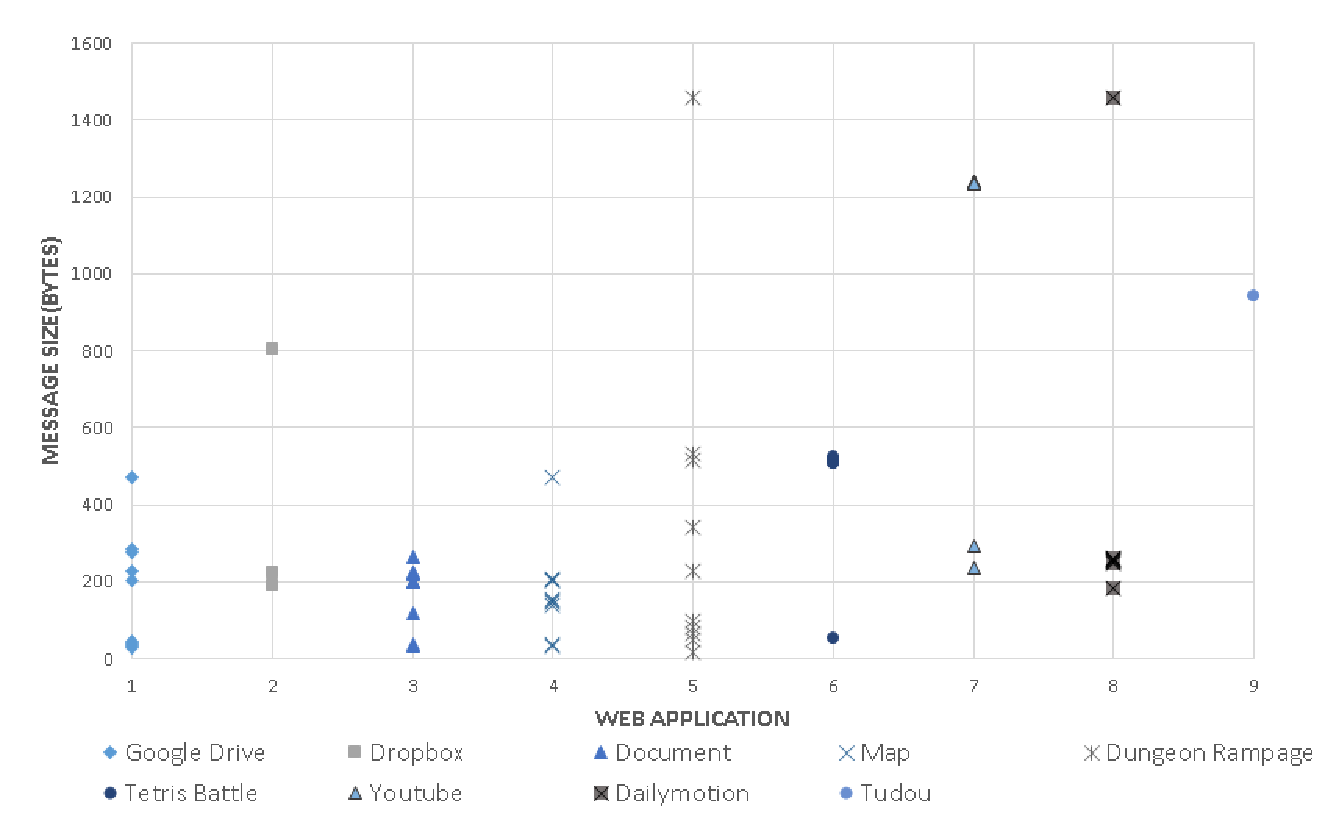
\includegraphics[width=1.0\textwidth]{msg_size_distribution1}
}\\
\subfloat[Firefox]{
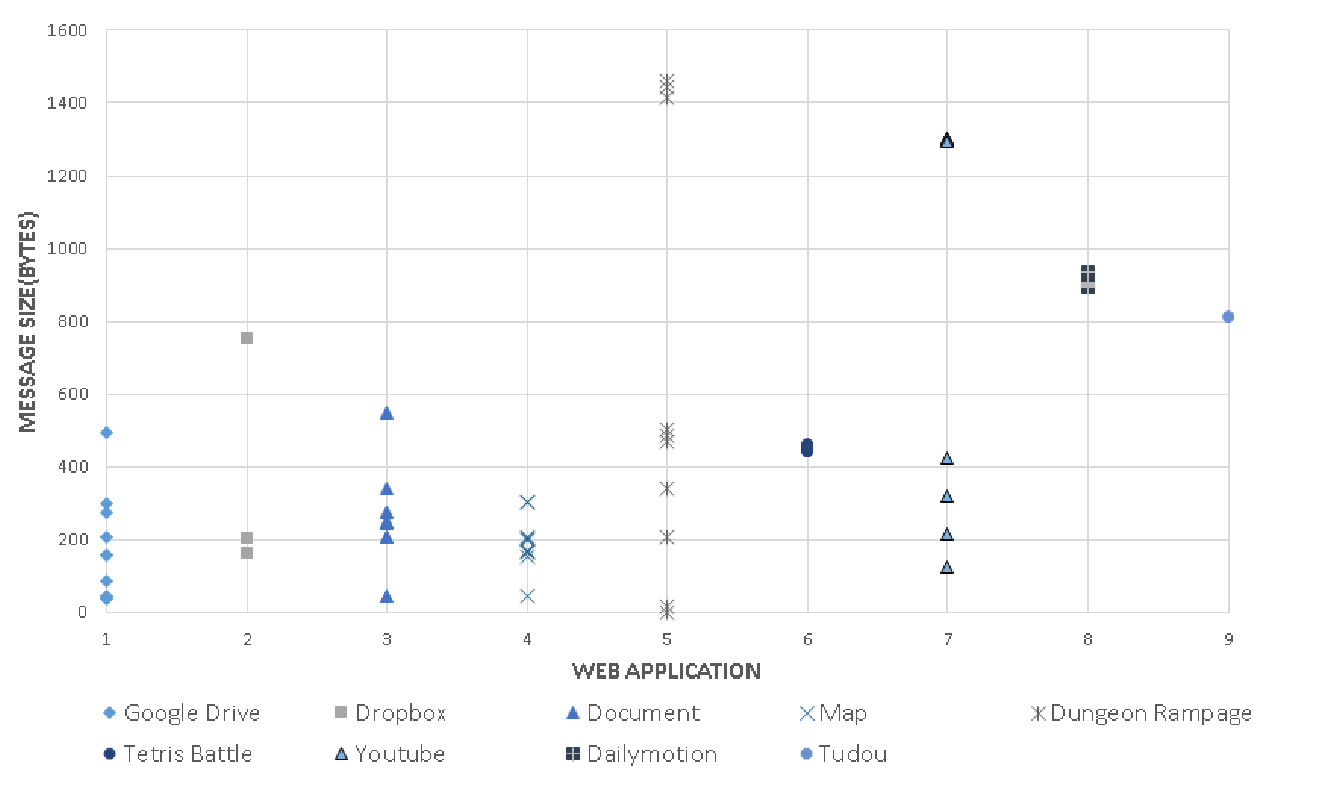
\includegraphics[width=1.0\textwidth]{msg_size_distribution2}
}
\caption{The message size distribution of each web application from two browsers.}
\label{Fig.msg_size_distribution}
\end{figure}

%底下這句的意思是我同樣是在做看影片的動作,但是用不同的平台來觀看會影響feature的結果
Performing the actions on similar web applications will result in different features. For example, the message size distribution of video streaming applications (Youtube, Dailymotion, Tudou) differ obviously according to Figure~\ref{Fig.msg_size_distribution}. However, we do not need to classify individual applications in practice because the management policies (e.g., bandwidth management or QoS) for similar applications are likely to be the same. Thus, we argue that it suffices to classify similar applications into the same category.

Figure~\ref{Fig.setlabel} shows the categorization procedure. We divide the web applications into five categories: file sharing, office, map, game and video streaming. A category consists of one or multiple similar applications. If an application is correctly classified, it is also classified into the correct category. Even though the features are occasionally ambiguous between the applications in the same category (e.g., Dailymotion and Tudou), the applications can be still classified into the category of video streaming applications.   

\begin{figure}[H]
\begin{center} 
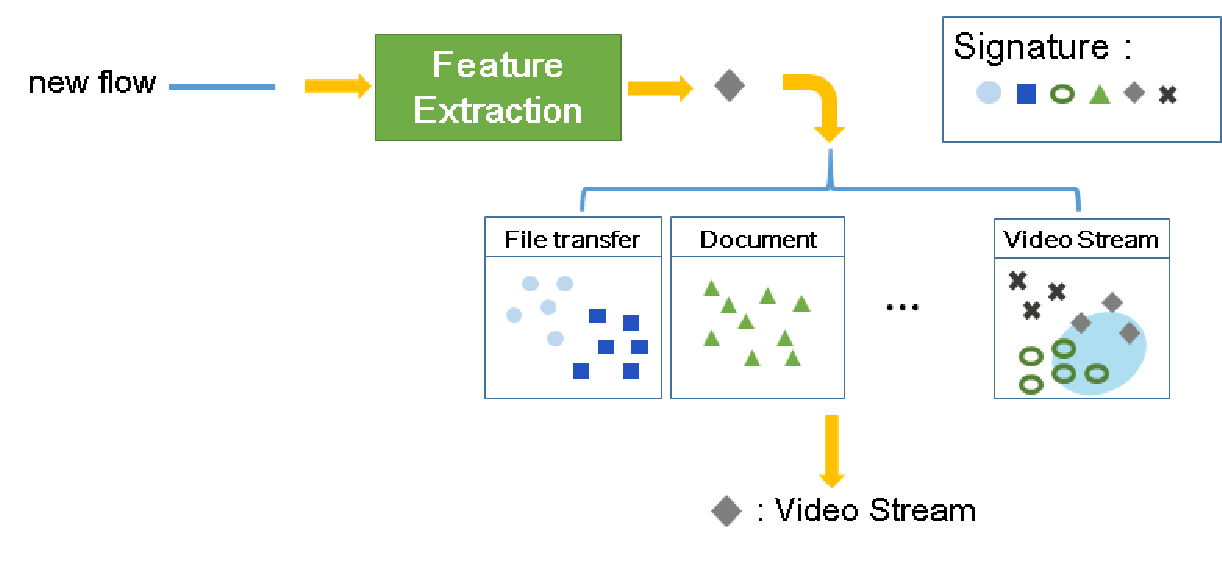
\includegraphics[width=1.0\textwidth]{setlabel}
\end{center}
\caption{Categorization of web applications.}
\label{Fig.setlabel}
\end{figure}


\section{Classification results}
\label{sec:result}
After we collect sufficient data from the browsers, we employ Weka to evaluate whether the feature is effective or not. Weka supports a collection of machine learning algorithms for data mining, among which we choose NBtree, Random Forest, J48graft and Naive Bayes to compare the classification accuracy by using different algorithms. We use 10-fold cross-validation to ensure the reliability. When testing the performance, we divide the web applications into two groups, i.e., interaction applications (document, map, game) and file transfer applications (video streaming, file transfer), since we want to compare the result with the previous method, which tests the accuracy of interaction applications and file transfer applications separately. In addition, the possibility of early classification is also evaluated and it will be described in detail on Section 4.4.4.

We choose the previous study to compare with our mechanism. Lin et al. presented the method based on fine-grained classification and used the average and the standard deviation of the request/response lengths as the features for classification. The difference between our targets is that we only want to classify the kinds of web applications; however, they want to distinguish what action a user does. In the work, they subdivide the flows into search keystrokes, editing, action and download. To dislodge the unnecessary message, they artificially input the first request time or the first request bytes. Nevertheless, that method is more suitable for offline analysis. The reason we choose this study as our comparison is that the way of features extraction ,which is independent of the network condition under the application layer, is similar to our mechanism.

\subsection{Classification with Similar Interactions in Each Run}
Table~\ref{table:inter_accuracy} shows the classification accuracy of each web application. The accuracy of all classifiers reach 95\% or above with our method, but the values still are slightly lower than previous work. There are some reasons may affect the result. For instance, our targets are different and we do not divide search keystroke messages from the flows we extract, since search packets and interaction packets may be transferred in the same connection. The true-positive rate in Google Map does not achieve 1 is because a few instances of Google Map are misidentified as those of Google document.


\begin{table}[H]
\centering
\caption{True/false positive rates of classifying the interactive connections.}
\label{table:inter_accuracy}
\begin{tabular}{|l|l|l|l|l|l|l|l|l|}
\hline
\multirow{2}{*}{} & \multicolumn{2}{l|}{\begin{tabular}[c]{@{}l@{}}Correctly \\ classified\\      (\%)\end{tabular}} 
				  & \multicolumn{2}{l|}{\begin{tabular}[c]{@{}l@{}}Document\\ \\    TP/FP\end{tabular}}                     
				  & \multicolumn{2}{l|}{\begin{tabular}[c]{@{}l@{}}Map \\     \\    TP/FP\end{tabular}}                   
				  & \multicolumn{2}{l|}{\begin{tabular}[c]{@{}l@{}}Game\\ \\              TP/FP\end{tabular}} \\ \cline{2-9} 
                  & Prior & New &Prior & New & Prior & New & Prior & New \\ \hline \hline
NBtree            & 99.80 & 97.50  & \begin{tabular}[c]{@{}l@{}}0.993/\\ 0.001\end{tabular} & \begin{tabular}[c]{@{}l@{}}1/\\ 0.033\end{tabular}   & \begin{tabular}[c]{@{}l@{}}0.999/\\ 0.005\end{tabular}    & 0.90/0  & 1/0    & 1/0  \\ \hline
RandomForest      & 99.89 & 98.75 & \begin{tabular}[c]{@{}l@{}}1/\\ 0.001\end{tabular}     & \begin{tabular}[c]{@{}l@{}}1/\\ 0.017\end{tabular}   & \begin{tabular}[c]{@{}l@{}}0.999/\\ 0\end{tabular}        & 0.95/0 & 1/0    & 1/0  \\ \hline
J48graft          & 99.28 & 97.50  & \begin{tabular}[c]{@{}l@{}}0.993/\\ 0.004\end{tabular} & \begin{tabular}[c]{@{}l@{}}1/\\ 0.033\end{tabular}   & \begin{tabular}[c]{@{}l@{}}0.996/\\ 0.019\end{tabular}    & 0.90/0  & 0.95/0 & 1/0  \\ \hline
NaiveBayes        & 99.49 & 95.00    & \begin{tabular}[c]{@{}l@{}}0.987/\\ 0\end{tabular}     & \begin{tabular}[c]{@{}l@{}}1/\\ 0.067\end{tabular}   & \begin{tabular}[c]{@{}l@{}}0.996/\\ 0.009\end{tabular}    & 0.80/0  & 1/0    & 1/0  \\ \hline
\multicolumn{9}{r}{Prior: Previous work / New : Our method}\\ 

\end{tabular}
\end{table}


%additional web applications
We also chose three additional web applications to disturb classification: Google sheets (type: document), Bing map (type: map) and Dungeon Blitz (type: game). We followed the scenarios described in Table~\ref{table:scenario_app}, and operated each web applications ten times on either Chrome or Firefox. We gathered the features generated from these additional applications and the original training set to verify the accuracy after the disturbance. The result is showed in Table~\ref{table:add_accuracy} and the accuracy after 10-fold cross-validation can be still up to 97.14\% for NBtree. In this work, we add additional applications only to the group of interaction applications to verify the accuracy because the variation of operations for file transfer applications are usually low.


\begin{table}[H]
\centering
\caption{True/false positive rates of classifying the interactive connections with additional web applications.}
\label{table:add_accuracy}
\begin{tabular}{|l|l|l|l|l|l|l|l|l|}
\hline
\multirow{2}{*}{} & \multicolumn{2}{l|}{\begin{tabular}[c]{@{}l@{}}Correctly\\ classified\\ (\%)\end{tabular}} & \multicolumn{2}{l|}{\begin{tabular}[c]{@{}l@{}}Document\\ \\ TP/FP\end{tabular}}                           & \multicolumn{2}{l|}{\begin{tabular}[c]{@{}l@{}}Map\\ \\ TP/FP\end{tabular}} & \multicolumn{2}{l|}{\begin{tabular}[c]{@{}l@{}}Game\\ \\ TP/FP\end{tabular}} \\ \cline{2-9} 
& Orig. & Add. & Orig. & Add. & Orig. & Add. & Orig. & Add.                                                           \\ \hline
NBtree            & 97.50                                       & 97.14                                       & \begin{tabular}[c]{@{}l@{}}1/\\ 0.033\end{tabular} & \begin{tabular}[c]{@{}l@{}}0.975/\\ 0.03\end{tabular} & 0.90/0        & \begin{tabular}[c]{@{}l@{}}0.925/\\ 0.01\end{tabular}       & 1/0          & 1/0                                                           \\ \hline
RandomRorest      & 98.75                                       & 95.71                                       & \begin{tabular}[c]{@{}l@{}}1/\\ 0.017\end{tabular} & \begin{tabular}[c]{@{}l@{}}0.95/\\ 0.04\end{tabular}  & 0.95/0        & \begin{tabular}[c]{@{}l@{}}0.90/\\ 0.02\end{tabular}        & 1/0          & 1/0                                                           \\ \hline
J48graft          & 97.50                                       & 92.14                                       & \begin{tabular}[c]{@{}l@{}}1/\\ 0.033\end{tabular} & \begin{tabular}[c]{@{}l@{}}0.90/\\ 0.06\end{tabular}  & 0.90/0        & \begin{tabular}[c]{@{}l@{}}0.85/\\ 0.04\end{tabular}        & 1/0          & \begin{tabular}[c]{@{}l@{}}0.983/\\ 0.013\end{tabular}        \\ \hline
NaiveBayes        & 95.00                                       & 95.71                                       & \begin{tabular}[c]{@{}l@{}}1/\\ 0.067\end{tabular} & \begin{tabular}[c]{@{}l@{}}0.975/\\ 0.05\end{tabular} & 0.80/0        & \begin{tabular}[c]{@{}l@{}}0.875/\\ 0.01\end{tabular}       & 1/0          & 1/0                                                           \\ \hline
\multicolumn{9}{r}{Orig.: Original training set / Add.: With additional web applications}\\


\end{tabular}
\end{table}


%file transfer applications
We also differentiate between downloading of video stream and general file transfer. We typed a video name and arbitrarily switched to multiple time positions when watching a video or just silently watched a video until the end on Youtube, Dailymotion and Tudou on the two browsers, but we up/downloaded files by Google drive and Dropbox. In summary, we watched 60 videos and transferred 40 files. After extracting the features, we used 10-fold cross-validation to evaluate the classification. It is presented in Table~\ref{table:file_accuracy} that the classification accuracy can be up to 97\% for all the classifiers, even better than previous work. 

\begin{table}[H]
\centering
\caption{True/false positive rates of classifying downloading connections.}
\label{table:file_accuracy}
\begin{tabular}{|l|l|l|l|l|l|l|}
\hline
\multirow{2}{*}{} & \multicolumn{2}{l|}{\begin{tabular}[c]{@{}l@{}}Correctly \\ classified\\ (\%)\end{tabular}} 
                  & \multicolumn{2}{l|}{\begin{tabular}[c]{@{}l@{}}Video\\ Streaming\\ TP/FP\end{tabular}}                    
                  & \multicolumn{2}{l|}{\begin{tabular}[c]{@{}l@{}}Files\\ Transfer\\ TP/FP\end{tabular}}       \\ \cline{2-7} 
& Prior & New & Prior & New & Prior & New  \\ \hline \hline
NBtree            & 92.72                                            & 97.00                                            & \begin{tabular}[c]{@{}l@{}}0.907/\\ 0\end{tabular} & \begin{tabular}[c]{@{}l@{}}0.967/\\ 0.025\end{tabular} & \begin{tabular}[c]{@{}l@{}}1/\\ 0.093\end{tabular} & \begin{tabular}[c]{@{}l@{}}0.975/\\ 0.033\end{tabular} \\ \hline
RandomForest      & 92.33                                            & 97.00                                            & \begin{tabular}[c]{@{}l@{}}0.902/\\ 0\end{tabular} & \begin{tabular}[c]{@{}l@{}}0.967/\\ 0.025\end{tabular} & \begin{tabular}[c]{@{}l@{}}1/\\ 0.098\end{tabular} & \begin{tabular}[c]{@{}l@{}}0.975/\\ 0.033\end{tabular} \\ \hline
J48graft          & 91.57                                            & 97.00                                            & \begin{tabular}[c]{@{}l@{}}0.893/\\ 0\end{tabular} & \begin{tabular}[c]{@{}l@{}}0.967/\\ 0.025\end{tabular} & \begin{tabular}[c]{@{}l@{}}1/\\ 0.107\end{tabular} & \begin{tabular}[c]{@{}l@{}}0.975/\\ 0.033\end{tabular} \\ \hline
NaiveBayes        & 92.72                                            & 97.00                                            & \begin{tabular}[c]{@{}l@{}}0.907/\\ 0\end{tabular} & \begin{tabular}[c]{@{}l@{}}0.967/\\ 0.025\end{tabular} & \begin{tabular}[c]{@{}l@{}}1/\\ 0.093\end{tabular} & \begin{tabular}[c]{@{}l@{}}0.975/\\ 0.033\end{tabular} \\ \hline
\multicolumn{7}{r}{Prior : Previous work / New : Our method}\\ 

\end{tabular}
\end{table}



\subsection{Classification with Diverse Interactions in Each Run}

In this subsection, instead of separating the web applications into interaction function and download function, we classify the traffic into five categories: document, map, game, video stream and file transfer. In the prior study of \cite{TFT14}, the authors evaluated classification separately because the features for interaction function and download function are different in that study, so we also separate the evaluation as well in the last subsection to compare with the prior study fairly. However, we use the same feature, i.e., top-5 most frequent message sizes from the requests, for all the web applications, so we classify all the categories for evaluation in this subsection. We also operated each web application ten times on either Chrome or Firefox, but deliberately performed an extremely different action in the same scenario. For example, we may just continuously type or intermittently edit a document for each time we collected in document function. The classification accuracy after 10-fold cross-validation also can be up to 93.89\% for Random Forest, meaning that the feature is stable and can be used for the classification with high accuracy. 

\begin{table}[H]
\centering
\caption{True/false positive rates of classifying all connections.}
\label{table:all_accuracy}
\begin{tabular}{|l|l|l|l|l|l|l|l|l|l|l|l|l|}
\hline
& \multicolumn{2}{l|}{\begin{tabular}[c]{@{}l@{}}Correctly \\ classified\\  (\%)\end{tabular}} 
& \multicolumn{2}{l|}{\begin{tabular}[c]{@{}l@{}}Document\\ \\ TP/FP\end{tabular}} 
& \multicolumn{2}{l|}{\begin{tabular}[c]{@{}l@{}}Map\\ \\ TP/FP\end{tabular}} 
& \multicolumn{2}{l|}{\begin{tabular}[c]{@{}l@{}}Game\\ \\ TP/FP\end{tabular}} 
& \multicolumn{2}{l|}{\begin{tabular}[c]{@{}l@{}}Video\\  Streaming\\    TP/FP\end{tabular}} 
& \multicolumn{2}{l|}{\begin{tabular}[c]{@{}l@{}}Files\\ Transfer\\ TP/FP\end{tabular}} \\ \hline \hline
NBtree       & \multicolumn{2}{l|}{92.22}                                                                       & \multicolumn{2}{l|}{\begin{tabular}[c]{@{}l@{}}1/\\ 0.05\end{tabular}}                 & \multicolumn{2}{l|}{\begin{tabular}[c]{@{}l@{}}0.80/\\ 0.006\end{tabular}}         & \multicolumn{2}{l|}{\begin{tabular}[c]{@{}l@{}}0.95/\\ 0.007\end{tabular}}   & \multicolumn{2}{l|}{\begin{tabular}[c]{@{}l@{}}0.917/\\ 0\end{tabular}}                  & \multicolumn{2}{l|}{\begin{tabular}[c]{@{}l@{}}0.925/\\ 0.029\end{tabular}}           \\ \hline
RandomForest & \multicolumn{2}{l|}{93.89}                                                                       & \multicolumn{2}{l|}{\begin{tabular}[c]{@{}l@{}}0.90/\\ 0.013\end{tabular}}              & \multicolumn{2}{l|}{\begin{tabular}[c]{@{}l@{}}0.90/\\ 0.019\end{tabular}}         & \multicolumn{2}{l|}{\begin{tabular}[c]{@{}l@{}}0.975/\\ 0.021\end{tabular}}  & \multicolumn{2}{l|}{\begin{tabular}[c]{@{}l@{}}0.933/\\ 0.017\end{tabular}}              & \multicolumn{2}{l|}{\begin{tabular}[c]{@{}l@{}}0.95/\\ 0.007\end{tabular}}            \\ \hline
J48graft     & \multicolumn{2}{l|}{92.22}                                                                       & \multicolumn{2}{l|}{\begin{tabular}[c]{@{}l@{}}0.95/\\ 0.031\end{tabular}}             & \multicolumn{2}{l|}{\begin{tabular}[c]{@{}l@{}}0.80/\\ 0.013\end{tabular}}         & \multicolumn{2}{l|}{\begin{tabular}[c]{@{}l@{}}0.975/\\ 0.021\end{tabular}}  & \multicolumn{2}{l|}{\begin{tabular}[c]{@{}l@{}}0.917/\\ 0.008\end{tabular}}              & \multicolumn{2}{l|}{\begin{tabular}[c]{@{}l@{}}0.925/\\ 0.021\end{tabular}}           \\ \hline
NaiveBayes   & \multicolumn{2}{l|}{92.22}                                                                       & \multicolumn{2}{l|}{\begin{tabular}[c]{@{}l@{}}0.95/\\ 0.025\end{tabular}}             & \multicolumn{2}{l|}{\begin{tabular}[c]{@{}l@{}}0.95/\\ 0.013\end{tabular}}        & \multicolumn{2}{l|}{\begin{tabular}[c]{@{}l@{}}0.95/\\ 0.029\end{tabular}}   & \multicolumn{2}{l|}{\begin{tabular}[c]{@{}l@{}}0.917/\\ 0.017\end{tabular}}              & \multicolumn{2}{l|}{\begin{tabular}[c]{@{}l@{}}0.875/\\ 0.014\end{tabular}}           \\ \hline
\end{tabular}
\end{table}

\subsection{Classification with Interactions from Multiple Users}

To ensure the accuracy does not too depend on specific users, we invited eight users to generate the traffic for the classification. In this subsection, we compare only interactive functions because the their actions are more diverse than download functions. The users were asked to perform similar actions to those from a single user and repeated three times for each web applications on Chrome and Firefox. The total number of packet traces is 192: 48 for Google document, 48 for Google map, 48 for Dungeon Rampage and 48 for Tetris Battle.

Table~\ref{table:multi_accuracy} shows the accuracy for each algorithm. We also used 10-fold cross-validation for this classification. The accuracy of our method for Naive Bayes is even higher than the results in Section 4.4, and can be up to 97.92\% with random forest. Compared the result with the training set shown in last subsection, the accuracy is degraded just slightly, meaning that the feature is stable. 

\begin{table}[H]
\centering
\caption{True/false positive rates of classifying the interactive connections for multiple users.}
\label{table:multi_accuracy}
\begin{tabular}{|l|l|l|l|l|l|l|l|l|}
\hline
\multirow{2}{*}{} & \multicolumn{2}{l|}{\begin{tabular}[c]{@{}l@{}}Correctly \\ classified\\      (\%)\end{tabular}} 
				  & \multicolumn{2}{l|}{\begin{tabular}[c]{@{}l@{}}Document\\ \\    TP/FP\end{tabular}}                     
				  & \multicolumn{2}{l|}{\begin{tabular}[c]{@{}l@{}}Map \\     \\    TP/FP\end{tabular}}                   
				  & \multicolumn{2}{l|}{\begin{tabular}[c]{@{}l@{}}Game\\ \\              TP/FP\end{tabular}} \\ \cline{2-9} 
                  & Prior & New & Prior & New & Prior & New & Prior & New \\ \hline \hline

NBtree            & 96.63                                        & 96.35                                        & \begin{tabular}[c]{@{}l@{}}0.939/\\ 0.025\end{tabular} & \begin{tabular}[c]{@{}l@{}}0.938/\\ 0.028\end{tabular} & \begin{tabular}[c]{@{}l@{}}0.971/\\ 0.044\end{tabular} & \begin{tabular}[c]{@{}l@{}}0.938/\\ 0.021\end{tabular} & \begin{tabular}[c]{@{}l@{}}0.993/\\ 0\end{tabular}     & 0.99/0                                                 \\ \hline
RandomForest     & 98.28                                        & 97.92                                        & \begin{tabular}[c]{@{}l@{}}0.954/\\ 0.009\end{tabular} & \begin{tabular}[c]{@{}l@{}}1/\\ 0.007\end{tabular}     & \begin{tabular}[c]{@{}l@{}}0.99/\\ 0.032\end{tabular}  & \begin{tabular}[c]{@{}l@{}}0.979/\\ 0.014\end{tabular} & 1/0                                                    & \begin{tabular}[c]{@{}l@{}}0.969/\\ 0.01\end{tabular}  \\ \hline
J48graft         & 97.65                                        & 93.75                                        & \begin{tabular}[c]{@{}l@{}}0.939/\\ 0.011\end{tabular} & \begin{tabular}[c]{@{}l@{}}0.917/\\ 0.035\end{tabular} & \begin{tabular}[c]{@{}l@{}}0.986/\\ 0.044\end{tabular} & \begin{tabular}[c]{@{}l@{}}0.917/\\ 0.035\end{tabular} & \begin{tabular}[c]{@{}l@{}}0.993/\\ 0.001\end{tabular} & \begin{tabular}[c]{@{}l@{}}0.958/\\ 0.021\end{tabular} \\ \hline
NaiveBayes       & 95.74                                        & 95.83                                        & \begin{tabular}[c]{@{}l@{}}0.87/\\ 0.017\end{tabular}  & \begin{tabular}[c]{@{}l@{}}0.938/\\ 0.028\end{tabular} & \begin{tabular}[c]{@{}l@{}}0.98/\\ 0.091\end{tabular}  & \begin{tabular}[c]{@{}l@{}}0.938/\\ 0.028\end{tabular} & \begin{tabular}[c]{@{}l@{}}1/\\ 0.001\end{tabular}     & \begin{tabular}[c]{@{}l@{}}0.979/\\ 0\end{tabular}     \\ \hline

\multicolumn{9}{r}{Pre: Previous work / New : Our method}\\ 

\end{tabular}
\end{table}


\subsection{Early Classification}
\label{sec:early}
The classification method in this work can be applied to manage various web applications, even though the web traffic is encrypted. The specifics of classification may vary in practice, depending on the purpose of management. If the purpose is accounting the usage of web applications in a network, it would suffice to classify the web applications offline based on the features from \emph{the entire packet traces} that have been observed. However, if the purpose is access control, classification after extracting the features from the entire packet traces will be too late to block the traffic in time. Thus, we also evaluate the effectiveness of early classification with the features from the partial messages in the beginning of the connections. In early classification, a connection can be blocked as soon as the web application is recognized based on the features from the partial messages. 

The packet traces for evaluating early classification are same as those described in the last subsection. We extracted the first $k$ messages from each main connection ($k=15, 20, 25, 30, 50, 100$) and used the size distribution of only these messages for the evaluation. Like the features from the entire packet traces, we also extracted the top five frequent message sizes in terms of occurrence frequency.  

The previous analysis show that the true-positive rate of almost all kinds of functions are at least up to 0.90; however, the true-positive rate for the map application is decreased to 0.80 because its features are not so stable as others. We choose Dungeon Rampage on Chrome as example for stable one shown as Figure~\ref{Fig.set_size_dr} and Google map on Chrome as example for unstable one shown as Figure~\ref{Fig.set_size_map}. The line chart is created by entire messages within a main connection and the scatter chart is created by the first $k$ messages in each figure.

\begin{figure}[H]
\begin{center} 
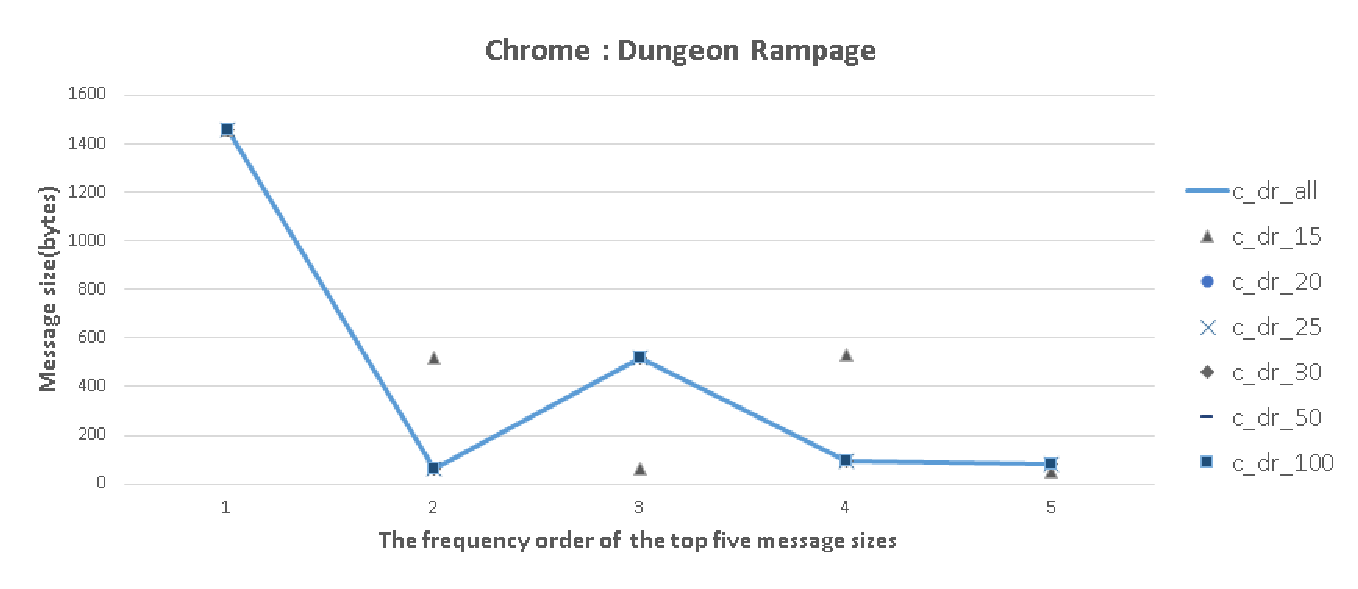
\includegraphics[width=1.1\textwidth]{early_dr}
\end{center}
\caption{The message size distribution for Dungeon Rampage.}
\label{Fig.set_size_dr}
\end{figure}

Figure~\ref{Fig.set_size_dr} depicts that the scatter charts are similar with the trend of line chart when we extract more than the first 20 messages. Figure~\ref{Fig.set_size_map} depicts that the scatter charts are almost similar with the trend of line chart when we extract more than the first 30 messages. So we finally extracted the first 30 messages from each web applications as our feature for early classification. The classification accuracy after 10-fold cross-validation can be at least 86.67\% and even can be up to 93.89\% for Random Forest.


\begin{figure}[H]
\begin{center} 
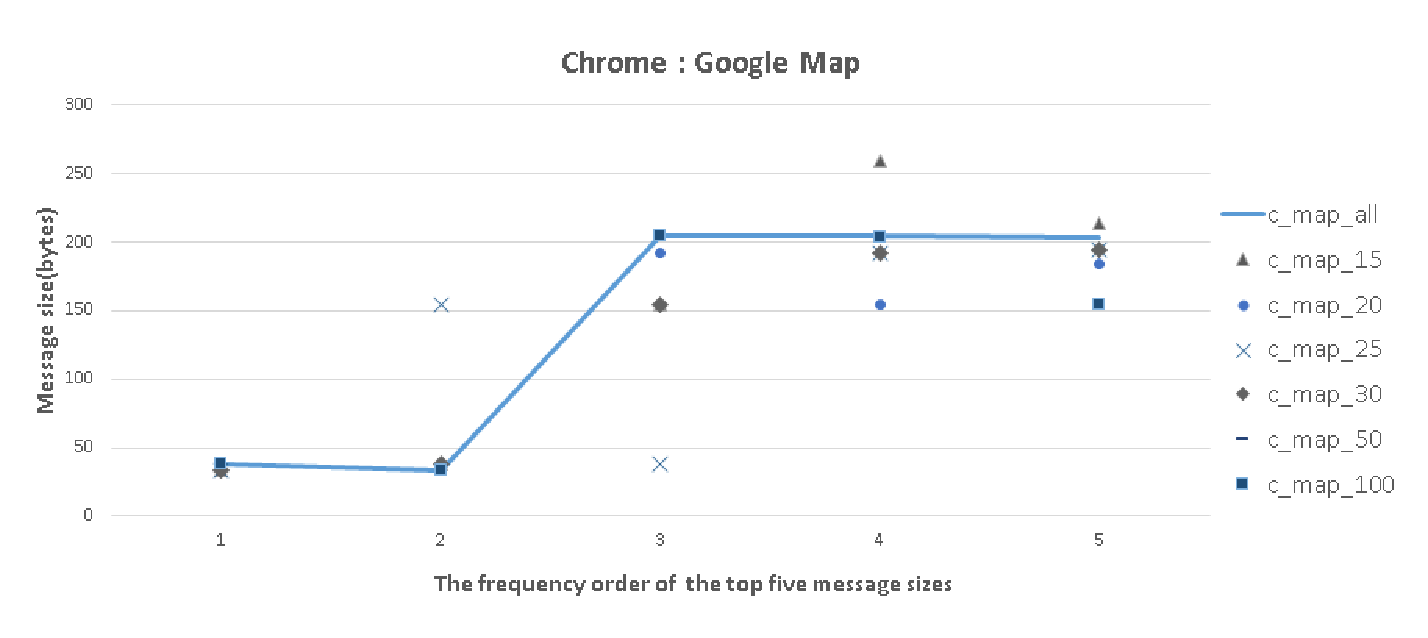
\includegraphics[width=1.1\textwidth]{early_map}
\end{center}
\caption{The message size distribution for Google map.}
\label{Fig.set_size_map}
\end{figure}

\begin{table}[H]
\centering
\caption{Early classification true/false positive rate in all connections.}
\label{table:early_accuracy}
\begin{tabular}{|l|l|l|l|l|l|l|}
\hline
& \begin{tabular}[c]{@{}l@{}}Correctly \\ classified\\ (\%)\end{tabular} 
& \begin{tabular}[c]{@{}l@{}}Document\\ \\ TP/FP\end{tabular} 
& \begin{tabular}[c]{@{}l@{}}Map \\ \\ TP/FP\end{tabular} 
& \begin{tabular}[c]{@{}l@{}}Game\\ \\ TP/FP\end{tabular} 
& \begin{tabular}[c]{@{}l@{}}Video\\ Stream\\ TP/FP\end{tabular} 
& \begin{tabular}[c]{@{}l@{}}File\\ Transfer\\ TP/FP\end{tabular} \\ \hline \hline
NBtree       & 86.67         & \begin{tabular}[c]{@{}l@{}}0.70/\\ 0.038\end{tabular}  & \begin{tabular}[c]{@{}l@{}}0.95/\\ 0.019\end{tabular}         & \begin{tabular}[c]{@{}l@{}}0.925/\\ 0.007\end{tabular}           & \begin{tabular}[c]{@{}l@{}}0.933/\\ 0.025\end{tabular} & \begin{tabular}[c]{@{}l@{}}0.75/\\ 0.079\end{tabular}           \\ \hline
RandomForest & 93.89         & \begin{tabular}[c]{@{}l@{}}0.85/\\ 0.013\end{tabular}  & 1/0                                                           & \begin{tabular}[c]{@{}l@{}}1/\\ 0.014\end{tabular}           & \begin{tabular}[c]{@{}l@{}}0.933/\\ 0.017\end{tabular} & \begin{tabular}[c]{@{}l@{}}0.90/\\ 0.036\end{tabular}           \\ \hline
J48graft     & 88.33         & \begin{tabular}[c]{@{}l@{}}0.85/\\ 0.019\end{tabular}  & \begin{tabular}[c]{@{}l@{}}1/\\ 0.019\end{tabular}            & \begin{tabular}[c]{@{}l@{}}0.95/\\ 0.029\end{tabular}           & \begin{tabular}[c]{@{}l@{}}0.85/\\ 0.042\end{tabular}  & \begin{tabular}[c]{@{}l@{}}0.825/\\ 0.043\end{tabular}          \\ \hline
NaïveBayes   & 87.22         & \begin{tabular}[c]{@{}l@{}}0.85/\\ 0.063\end{tabular}  & \begin{tabular}[c]{@{}l@{}}0.95\\ /0.013\end{tabular}         & \begin{tabular}[c]{@{}l@{}}0.925/\\ 0.021\end{tabular}           & \begin{tabular}[c]{@{}l@{}}0.95/\\ 0.017\end{tabular}  & \begin{tabular}[c]{@{}l@{}}0.675/\\ 0.043\end{tabular}          \\ \hline
\end{tabular}
\end{table}

\section{Practice and Limitation}
\label{sec:app_limit}

Even though the classification accuracy is high for extracted packet traces from real user interactions with web applications, there are still some issues that should be addressed to deploy this classification in practice.

First, although one IP address may be associated with more than one web application, as we demonstrated earlier in this work, we can still record the mapping between the IP addresses and their associated applications from earlier classification in a list to speed up classification. Since the mapping may be one-to-many, if a remote IP address can be found in the list and it is mapped to only one application, we can leverage the result of earlier classification to label the traffic to that application directly; otherwise, we can follow the procedure described in Chapter 3 to classify the web application. The result from earlier classification can at least help reduce the scope of possible labels.

Second, the traffic for each packet trace is just generated from a specific web application in this work, but in reality, we will need to analyze multiple applications at the same time and extracting the main connection is a problem. To solve this issue, we will observe the traffic density and quantity of each IP address during a period time and if the values both reach the thresholds, we will extract it as the main connection for classification. After classification, if the device that employs the design determines to block the main connection, the connections having the same pair of source/destination IP addresses as the main connection and happening around it will be blocked as well. Furthermore, users may use a web application not in the training set. Thus, after traffic classification, we will have to compute the distance between the feature vectors of the analyzed traffic and the application(s) that the analyzed traffic is supposed to be. If the distance is too long, than the analyzed traffic will be labeled as unknown.


Third, if the main connection is identified after the web application has been executed for a period of time, it may be too late to block an application for access control since the function is likely to have already completed its execution when the flows are collected and analyzed. The early classification described in Section~\ref{sec:early} can address this issue. Moreover, the accuracy may be decreased if the execution time of an web application function is too short to extract meaningful feature. 
